%# -*- coding: utf-8-unix -*-
%%==================================================
\chapter{流体力学}
\label{chap1}
\begin{itemize}[noitemsep,topsep=0pt,parsep=0pt,partopsep=0pt]
	\item ...
\end{itemize}

\section{知识点和方法论}


\subsection{流体力学需要遵守的三个物理学原理}

1. 质量守恒定律

2. 牛顿第二定律(力 = 质量 $\times$ 加速度)

3. 能量守恒定律

\subsection{流体力学基本控制方程}

1. 连续性方程

2. 动量方程

3. 能量方程

\subsection{流体力学流动模型}

1. 固定的有限控制体, 直接导出守恒型积分方程

2. 移动的有限控制体, 直接导出非守恒型积分方程

3. 固定的无穷小控制体, 直接导出守恒型偏微分方程

4. 移动的无穷小控制体(移动的流动微团), 直接导出非守恒型偏微分方程

\subsection{条件}
1. 边界条件

2. 无粘流

3. 粘性流

\subsection{速度向量场}

$\vec{V} = u\vec{i} + v\vec{j} + w\vec{k}$

速度分量

u = u(x, y, z, t)

v = v(x, y, z, t)

w = w(x, y, z, t)

\subsection{标量密度场}

$\rho = \rho (x_1, y_1, z_1, t_1)$

\subsection{物质导数}

$\lim _{t_2 -> t_1} \frac{\rho_2 - \rho_1}{t_2 - t1} = \frac{D\rho}{Dt}$

密度的物质导数就是, 流体微团在空间运动时, 其密度的时间变化率.  它和偏导数$\partial \rho / \partial t$ 不同, 偏导数表示的是在固定位置点的变量率.

$\frac{D\rho}{Dt} = \frac{\partial \rho}{\partial t} + u \frac{\partial \rho}{\partial x} + v \frac{\partial \rho}{\partial y} + w \frac{\partial \rho}{\partial z}$

笛卡尔坐标系下向量算子$\nabla = \vec{i} \frac{\partial}{\partial x} + \vec{j} \frac{\partial}{\partial y} + k \frac{\partial}{ \partial z}$

物质导数 则为 $\frac{D}{Dt} = \frac{\partial}{\partial t} + \vec{V} \cdot \nabla$

$\frac{\partial}{\partial t}$ 叫做当地导数, 它在物理上是固定点出的时间变化率.

$\vec{V} \cdot \nabla$ 叫做迁移导数, 它在物理上表示由于流体微团从刘长忠的一点运动到另一点, 流畅度额空间不均匀性而引起的时间变化率.

物质导数和时间的全导数是相同的.

\subsection{速度散度}

$\nabla \cdot \vec{V} = \frac{1}{\delta \mathcal{V} } \frac{D(\delta \mathcal{V})}{Dt}$

右边就是速度散度, 左边就是速度散度的物理意义, 即 $\nabla \cdot \vec{V}$ 是每单位体积运动着的流体微团, 体积相对变化的时间变化率.

\subsection{空间位置固定的有限控制体模型}
通过控制面S流出控制体的净质量流量(B) = 控制体内质量减少的时间变化率(C)

通过面积dS的质量流量微元为 $\rho \vec{V_n} dS = \rho \vec{V} \cdot d\vec{S}$

$d \vec{S}$ 的方向总是指向控制体外. 当$\vec{V}$ 也指向控制体外, 表示质量流量在物理上是离开控制体的, 也就是流出. 因此,

$$
	B = \iint_{S} \rho V \cdot d\vec{S}
$$

$$
	C = - \frac{\partial}{\partial t}\iiint_{\mathcal{V} \rho d \mathcal{V}}
$$

$$
	B + C = 0
$$
是连续性方程的积分形式. 控制体有限的体积就是方程具有积分形式的原因.


\subsection{随流体运动的有限控制体模型}
该控制体优势有相同的, 可辨认的质量微团组成. 也就是说, 这种运动的控制体具有固定不变的质量.

有限控制体的总质量 =
$$
	m = \iiint_{\mathcal{V}} \rho d \mathcal{V}
$$

整个控制体的质量的物质导数为0

$$
	\frac{D}{Dt} \iiint_{\mathcal{V}} \rho d \mathcal{V} = 0
$$

\subsection{空间位置固定的无穷小微团模型}

我们定义净流出量为正

那么我们有, x 方向的净流出量
$$
	[ \rho u + \frac{\partial (\rho u)}{\partial x} ] dy dz - (\rho u) dydz = \frac{\partial (\rho u)}{\partial x} dxdydz
$$

y 方向的净流出量

$$
	[ \rho v + \frac{\partial (\rho v)}{\partial y} ] dx dz - (\rho v) dxdz = \frac{\partial (\rho v)}{\partial y} dxdydz
$$

z 方向的净流出量

$$
	[ \rho w + \frac{\partial (\rho w)}{\partial z} ] dx dy - (\rho w) dxdy = \frac{\partial (\rho w)}{\partial z} dxdydz
$$

那么净流出量 $$=[\frac{\partial (\rho w)}{\partial z} + \frac{\partial (\rho v)}{\partial y} + \frac{\partial (\rho u)}{\partial x} ] dxdydz$$

微团的总质量是 $\rho (dxdydz)$ , 因此微团内质量增加的时间变化率为 = $\frac{\partial \rho}{\partial t} (dxdydz)$


根据质量守恒定律

$$
	[\frac{\partial (\rho w)}{\partial z} + \frac{\partial (\rho v)}{\partial y} + \frac{\partial (\rho u)}{\partial x} ] dxdydz = -\frac{\partial \rho}{\partial t} (dxdydz)
$$

=>

$$
	\frac{\partial \rho}{\partial t}  + [\frac{\partial (\rho w)}{\partial z} + \frac{\partial (\rho v)}{\partial y} + \frac{\partial (\rho u)}{\partial x} ] = 0
$$

=>

$$
	\frac{\partial \rho}{\partial t} + \nabla \cdot (\rho \vec{V}) = 0
$$

上述方程式连续性方程的偏微分方程形式. 他是基于空间位置固定的无穷小微团模型.

\subsection{随流体运动的无穷小微团模型}
这个流体微团有固定的质量, 但它的形状和体积会在它向下游运动时变化. 将这个流体微团固定的质量和可变的体积分别用 $\delta m$ 和 $\delta \mathcal{V}$ 表示.

=>

$$
	\delta m = \rho \delta \mathcal{V}
$$

他的质量随时间的变化率为0

$$
	\frac{D(\delta m)}{Dt} = 0
$$

=>

$$
	\frac{D(\rho \delta \mathcal{V})}{Dt} = \delta \mathcal{V} \frac{D\rho}{Dt} + \rho \frac{D(\delta \mathcal{V})}{Dt} = 0
$$

=>

$$
	\frac{D\rho}{Dt} + \rho \nabla \cdot \vec{V} = 0
$$

上式是连续性方程的另一种偏微分方程的形式, 由岁流体运动额流动模型直接导出的控制方程定义为非守恒型方程.

\subsection{散度定理}
简单来说就是把面积分转为体积分, 也要求数学上的连续性

$$
	\iint_{S}(p\mathcal{V})\cdot d\vec{S} = \iiint_{\mathcal{V}} \nabla \cdot (\rho \vec{V}) d \mathcal{V}
$$
\subsection{对于标量与向量成绩的散度, 有向量恒等式}

$$
	\nabla \cdot (\rho \vec{V}) = (\rho \nabla \cdot \vec{V}) + (\vec{V} \cdot \nabla \rho)
$$

也就是说, 一个标量与一个向量成绩的散度等于标量与向量散度的成绩加上向量与标量梯度的点积.
\subsection{动量方程}

$$
	\vec{F}_{x} = m \vec{a}_x
$$

x方向的动量方程

有两种里会影响真个流体微团, 体积力, 直接作用在流体微团整个体积委员上的力, 而且租用是超距离的, 比如重力, 电场力, 磁场力.

表面力, 直接作用在流体微团的表面, 他们只能由两种原因引起: 1. 由包在流体微团周围的流体所施加的, 作用于微团表面的压力分布; 2. 由于外部流体推拉微团而产生的, 以摩擦的方式作用于表面的切应力和正应力
分布.

x轴方向总的表面力 = $$
	[p-(p+\frac{\partial p}{\partial x}dx)]dydz + [(\tau_{xx} + \frac{\partial \tau_{xx}}{\partial x} - \tau_{xx} )]dydz +
	[(\tau_{yz} + \frac{\partial \tau_{yz}}{\partial y} dy) - \tau _{yz}]dxdz + [(\tau_zx + \frac{\partial \tau_{zx}}{\partial z}dz) - \tau_{rz}]dxdy
$$
里面含有压力和切应力



作用在单位质量流体微团上的体积力记作$\mathcal{f}$, 其x方向分量为$\mathcal{f}_x$. 流体微团的体积为dxdydz, 所以LinkedList还可以当做队列来使用

作用在流体微团上的体积力的x方向风量=$\rho \mathcal{f}_x(dxdydz)$

x方向总的力$F_x$

$$
	F_x=(-\frac{\partial p}{\partial x} + \frac{\partial \tau_{xx}}{\partial x} + \frac{\partial \tau_{yx}}{\partial y} +
	\frac{\partial \tau_{zx}}{\partial z})dxdydz + \rho \mathcal{f}_xdxdydz = ma = \rho \frac{Du}{Dt} dxdydz
$$

=>

$$
	\rho \frac{Dv}{Dt} = -\frac{\partial p}{\partial y} + \frac{\partial \tau_{xy}}{\partial x} + \frac{\partial \tau_{yy}}{\partial y} + \frac{\partial \tau_{zy}}{\partial  z} + \rho \mathcal{f}_y
$$

$$
	\rho \frac{Dw}{Dt} = -\frac{\partial p}{\partial z} + \frac{\partial \tau_{xz}}{\partial x} + \frac{\partial \tau_{yz}}{\partial y} + \frac{\partial \tau_{zz}}{\partial  z} + \rho \mathcal{f}_z
$$

上述三个方程也统称为N-V方程. 纳维-斯托克斯方程.

=>

$$
	\frac{\partial (\rho u)}{\partial t} + \nabla \cdot (\rho u \vec{V}) = (-\frac{\partial p}{\partial x} + \frac{\partial \tau_{xx}}{\partial x} + \frac{\partial \tau_{yx}}{\partial y} +
	\frac{\partial \tau_{zx}}{\partial z}) + \rho \mathcal{f}_x
$$

$$
	\frac{\partial (\rho v)}{\partial t} + \nabla \cdot (\rho v \vec{V}) = (-\frac{\partial p}{\partial y} + \frac{\partial \tau_{xy}}{\partial x} + \frac{\partial \tau_{yy}}{\partial y} +
	\frac{\partial \tau_{zy}}{\partial z}) + \rho \mathcal{f}_y
$$

$$
	\frac{\partial (\rho w)}{\partial t} + \nabla \cdot (\rho w \vec{V}) = (-\frac{\partial p}{\partial z} + \frac{\partial \tau_{xz}}{\partial x} + \frac{\partial \tau_{yz}}{\partial y} +
	\frac{\partial \tau_{zz}}{\partial z}) + \rho \mathcal{f}_z
$$

牛顿流体: 流体的切应力与应变的时间变化率, 也就是速度梯度, 是成正比的.

空气动力学中都是牛顿流体.

$$
	\tau_{xx} = \lambda (\nabla \cdot \vec{V}) + 2\mu \frac{\partial u}{\partial x}
$$

$$
	\tau_{yy} = \lambda(\nabla \cdot \vec{V}) + 2 \mu \frac{\partial v}{\partial y}
$$

$$
	\tau_{zz} = \lambda(\nabla \cdot \vec{V}) + 2 \mu \frac{\partial w}{\partial y}
$$

$$
	\tau_{xy} = \tau_{yx} =   \mu (\frac{\partial v}{\partial x} + \frac{\partial u}{ \partial y})
$$

$$
	\tau_{xz} = \tau_{zx} =   \mu (\frac{\partial u}{\partial z} + \frac{\partial w}{ \partial x})
$$

$$
	\tau_{yz} = \tau_{zy} =   \mu (\frac{\partial w}{\partial y} + \frac{\partial v}{ \partial z})
$$
其中, $\mu$ 是分子粘性系数, $\lambda$ 是第二粘性系数. 斯托克斯提出假设

$$
	\lambda = -\frac{2}{3} \mu
$$

=> 完整的NV守恒方程

$$
	\frac{\partial (\rho u)}{\partial t} + \frac{\partial (\rho u^2)}{\partial x} + \frac{\partial(\rho uv)}{ \partial y} + \frac{\partial (\rho u w)}{\partial z} =
	-\frac{\partial p}{\partial x} + \frac{\partial}{\partial t}(\lambda \nabla \cdot \vec{V} + 2\mu \frac{\partial u}{\partial x}) +
	\frac{\partial }{\partial y}[\mu(\frac{\partial v}{\partial x} + \frac{\partial u}{\partial y})] +
	\frac{\partial}{\partial z}[\mu(\frac{\partial u}{\partial z} + \frac{\partial w}{\partial x})] + \rho \mathcal{f}_x
$$

$$
	\begin{gathered}
		\frac{\partial(\rho v)}{\partial t}+\frac{\partial(\rho u v)}{\partial x}+\frac{\partial\left(\rho v^{2}\right)}{\partial y}+\frac{\partial(\rho v w)}{\partial z}=-\frac{\partial p}{\partial y}+\frac{\partial}{\partial x}\left[\mu\left(\frac{\partial v}{\partial x}+\frac{\partial u}{\partial y}\right)\right]+ \\
		\frac{\partial}{\partial y}\left(\lambda \nabla \cdot V+2 \mu \frac{\partial v}{\partial y}\right)+\frac{\partial}{\partial z}\left[\mu\left(\frac{\partial w}{\partial y}+\frac{\partial v}{\partial z}\right)\right]+\rho f_{y}
	\end{gathered}
$$

$$
	\frac{\partial(\rho w)}{\partial t}+\frac{\partial(\rho u w)}{\partial x}+\frac{\partial(\rho v w)}{\partial y}+\frac{\partial\left(\rho w^{2}\right)}{\partial z}=-\frac{\partial p}{\partial z}+\frac{\partial}{\partial x}\left[\mu\left(\frac{\partial u}{\partial z}+\frac{\partial w}{\partial x}\right)\right]+ \\
	\frac{\partial}{\partial y}\left[\mu\left(\frac{\partial w}{\partial y}+\frac{\partial v}{\partial z}\right)\right]+\frac{\partial}{\partial z}\left(\lambda \nabla \cdot V+2 \mu \frac{\partial w}{\partial z}\right)+\rho f_{z}
$$
\subsection{能量方程}

流体微团内能量的变化率=流入微团内的净热流量+体积力和表面力对微团做功的功率

A = B + C

C为, 对物体做功的功率等于这个力乘以速度在此力作用方向的分量.

$$
	\rho \mathcal{f} \cdot \vec{V} (dxdydz)
$$

压力在x方向做功的功率为

$$
	\left[u p-\left(u p+\frac{\partial(u p)}{\partial x} \mathrm{~d} x\right)\right] \mathrm{d} y \mathrm{~d} z=-\frac{\partial(u p)}{\partial x} \mathrm{~d} x \mathrm{~d} y \mathrm{~d} z
$$


切应力在x方向上做功的功率是

$$
	\left[\left(u \tau_{y x}+\frac{\partial\left(u \tau_{y x}\right)}{\partial y} \mathrm{~d} y\right)-u \tau_{y x}\right] \mathrm{d} x \mathrm{~d} z=\frac{\partial\left(u \tau_{y x}\right)}{\partial y} \mathrm{~d} x \mathrm{~d} y \mathrm{~d} z
$$

所有表面力x方向的做功的和

$$
	\left[-\frac{\partial(u p)}{\partial x}+\frac{\partial\left(u \tau_{x x}\right)}{\partial x}+\frac{\partial\left(u \tau_{y x}\right)}{\partial y}+\frac{\partial\left(u \tau_{z x}\right)}{\partial z}\right] \mathrm{d} x \mathrm{~d} y \mathrm{~d} z
$$

xyz方向上的做功和

$$
	\begin{aligned}
		C= & -\left[\left(\frac{\partial(u p)}{\partial x}+\frac{\partial(v p)}{\partial y}+\frac{\partial(w p)}{\partial z}\right)+\frac{\partial\left(u \tau_{x x}\right)}{\partial x}+\frac{\partial\left(u \tau_{y x}\right)}{\partial y}+\frac{\partial\left(u \tau_{z x}\right)}{\partial z}+\frac{\partial\left(v \tau_{x y}\right)}{\partial x}+\right.                                    \\
		   & \left.\frac{\partial\left(v \tau_{r y}\right)}{\partial y}+\frac{\partial\left(v \tau_{z y}\right)}{\partial z}+\frac{\partial\left(w \tau_{z z}\right)}{\partial x}+\frac{\partial\left(w \tau_{y z}\right)}{\partial y}+\frac{\partial\left(w \tau_{z}\right)}{\partial z}\right] \mathrm{d} x \mathrm{~d} y \mathrm{~d} z+\rho f \cdot V \mathrm{~d} x \mathrm{~d} y \mathrm{~d} z
	\end{aligned}
$$

$\dot{q}$ 定义为单位质量的体积加热率.

微团的体积加热(吸收或释放的辐射热) = $\dot{q} \rho dxdydz$

$$
	\text { 热传导对流体微团的加热 }=-\left(\frac{\partial \dot{q}_{x}}{\partial x}+\frac{\partial \dot{q}_{y}}{\partial y}+\frac{\partial \dot{q}_{z}}{\partial z}\right) \mathrm{d} x \mathrm{~d} y \mathrm{~d} z
$$

$$
	B=\left[\rho \dot{q}-\left(\frac{\dot{\partial} \dot{q}_{x}}{\partial x}+\frac{\partial \dot{q}_{y}}{\partial y}+\frac{\partial \dot{q}_{z}}{\partial z}\right)\right] \mathrm{d} x \mathrm{~d} y \mathrm{~d} z
$$

根据傅里叶热传导定律, 热传导产生的热流与当地的问题梯度成正比

$$
	\dot{q}_{x}=-k \frac{\partial T}{\partial x} \quad \dot{q}_{y}=-k \frac{\partial T}{\partial y} \quad \dot{q}_{z}=-k \frac{\partial T}{\partial z}
$$

k 为 热导率

=>

$$
	B=\left[\rho \dot{q}+\frac{\partial}{\partial x}\left(k \frac{\partial T}{\partial x}\right)+\frac{\partial}{\partial y}\left(k \frac{\partial T}{\partial y}\right)+\frac{\partial}{\partial z}\left(k \frac{\partial T}{\partial z}\right)\right] \mathrm{d} x \mathrm{~d} y \mathrm{~d} z
$$

流体微团内能量= 由于分子随机运动而产生的(单位质量)内能$e$ + 流体微团平动是具有的动能. 单位质量的动能为 $V^2 / 2$

单位质量的总能量变化的时间变化率由物质导数给出.

$$
	A=\rho \frac{D}{D t}\left(e+\frac{V^{2}}{2}\right) \mathrm{d} x \mathrm{~d} y \mathrm{~d} z
$$

=> 总公式

$$
	\begin{aligned}
		\rho \frac{\mathrm{D}}{\mathrm{D} t}\left(e+\frac{V^{2}}{2}\right)= & \rho \dot{q}+\frac{\partial}{\partial x}\left(k \frac{\partial T}{\partial x}\right)+\frac{\partial}{\partial y}\left(k \frac{\partial T}{\partial y}\right)+\frac{\partial}{\partial z}\left(k \frac{\partial T}{\partial z}\right)-                                                                                                        \\
		                                                                    & \frac{\partial(u p)}{\partial x}-\frac{\partial(v p)}{\partial y}-\frac{\partial(w p)}{\partial z}+\frac{\partial\left(u \tau_{x x}\right)}{\partial x}+\frac{\partial\left(u \tau_{y x}\right)}{\partial y}+\frac{\partial\left(u \tau_{z x}\right)}{\partial z}+                                                                           \\
		                                                                    & \frac{\partial\left(v \tau_{x y}\right)}{\partial x}+\frac{\partial\left(v \tau_{y y}\right)}{\partial y}+\frac{\partial\left(v \tau_{z y}\right)}{\partial z}+\frac{\partial\left(w \tau_{x z}\right)}{\partial x}+\frac{\partial\left(w \tau_{y z}\right)}{\partial y}+\frac{\partial\left(w \tau_{z z}\right)}{\partial z}+\rho f \cdot V
	\end{aligned}
$$

=> 将方程左边只包含内能

$$
	\begin{gathered}
		\rho \frac{\mathrm{D} e}{\mathrm{D} t}=\rho \dot{q}+\frac{\partial}{\partial x}\left(k \frac{\partial T}{\partial x}\right)+\frac{\partial}{\partial y}\left(k \frac{\partial T}{\partial y}\right)+\frac{\partial}{\partial z}\left(k \frac{\partial T}{\partial z}\right)-p\left(\frac{\partial u}{\partial x}+\frac{\partial v}{\partial y}+\frac{\partial w}{\partial z}\right)+ \\
		\tau_{x x} \frac{\partial u}{\partial x}+\tau_{y x} \frac{\partial u}{\partial y}+\tau_{z z} \frac{\partial u}{\partial z}+\tau_{x y} \frac{\partial v}{\partial x}+\tau_{y y} \frac{\partial v}{\partial y}+\tau_{z y} \frac{\partial v}{\partial z}+\tau_{x z} \frac{\partial w}{\partial x}+\tau_{y z} \frac{\partial w}{\partial y}+\tau_{z z} \frac{\partial w}{\partial z}
	\end{gathered}
$$

=> 利用 $\tau_{xy} == \tau_{yx} ...$


$$
	\begin{gathered}
		\rho \frac{\mathrm{D} e}{\mathrm{D} t}=\rho \dot{q}+\frac{\partial}{\partial x}\left(k \frac{\partial T}{\partial x}\right)+\frac{\partial}{\partial y}\left(k \frac{\partial T}{\partial y}\right)+\frac{\partial}{\partial z}\left(k \frac{\partial T}{\partial z}\right)-p\left(\frac{\partial u}{\partial x}+\frac{\partial v}{\partial y}+\frac{\partial w}{\partial z}\right)+ \\
		\lambda\left(\frac{\partial u}{\partial x}+\frac{\partial v}{\partial y}+\frac{\partial w}{\partial z}\right)^{2}+\mu\left[2\left(\frac{\partial u}{\partial x}\right)^{2}+2\left(\frac{\partial v}{\partial y}\right)^{2}+2\left(\frac{\partial w}{\partial z}\right)^{2}+\right. \\
			\left.\left(\frac{\partial u}{\partial y}+\frac{\partial v}{\partial x}\right)^{2}+\left(\frac{\partial u}{\partial z}+\frac{\partial w}{\partial x}\right)^{2}+\left(\frac{\partial v}{\partial z}+\frac{\partial w}{\partial y}\right)^{2}\right]
	\end{gathered}
$$


=> 内能表示的守恒型能量方程

$$
	\begin{aligned}
		\frac{\partial(\rho e)}{\partial t}+\nabla \cdot(\rho e V)= & \rho \dot{q}+\frac{\partial}{\partial x}\left(k \frac{\partial T}{\partial x}\right)+\frac{\partial}{\partial y}\left(k \frac{\partial T}{\partial y}\right)+\frac{\partial}{\partial z}\left(k \frac{\partial T}{\partial z}\right)-               \\
		                                                            & p\left(\frac{\partial u}{\partial x}+\frac{\partial v}{\partial y}+\frac{\partial w}{\partial z}\right)+\lambda\left(\frac{\partial u}{\partial x}+\frac{\partial v}{\partial y}+\frac{\partial w}{\partial z}\right)^{2}+                          \\
		                                                            & \mu\left[2\left(\frac{\partial u}{\partial x}\right)^{2}+2\left(\frac{\partial v}{\partial y}\right)^{2}+2\left(\frac{\partial w}{\partial z}\right)^{2}+\right.                                                                                    \\
		                                                            & \left.\left(\frac{\partial u}{\partial y}+\frac{\partial v}{\partial x}\right)^{2}+\left(\frac{\partial u}{\partial z}+\frac{\partial w}{\partial x}\right)^{2}+\left(\frac{\partial v}{\partial z}+\frac{\partial w}{\partial y}\right)^{2}\right]
	\end{aligned}
$$


=>总能量表示的守恒型方程

$$
	\begin{aligned}
		  & \frac{\partial}{\partial t}\left[\rho\left(e+\frac{V^{2}}{2}\right)\right]+\nabla \cdot\left[\rho\left(e+\frac{V^{2}}{2}\right) V\right]                                                                                                                                                                                                 \\
		= & \rho \dot{q}+\frac{\partial}{\partial x}\left(k \frac{\partial T}{\partial x}\right)+\frac{\partial}{\partial y}\left(k \frac{\partial T}{\partial y}\right)+\frac{\partial}{\partial z}\left(k \frac{\partial T}{\partial z}\right)-\frac{\partial(u p)}{\partial x}-\frac{\partial(v p)}{\partial y}-\frac{\partial(w p)}{\partial z}+ \\
		  & \frac{\partial\left(u \tau_{x x}\right)}{\partial x}+\frac{\partial\left(u \tau_{y x}\right)}{\partial y}+\frac{\partial\left(u \tau_{z x}\right)}{\partial z}+\frac{\partial\left(v \tau_{x y}\right)}{\partial x}+\frac{\partial\left(v \tau_{y y}\right)}{\partial y}+\frac{\partial\left(u \tau_{x y}\right)}{\partial z}+           \\
		  & \frac{\partial\left(w \tau_{x z}\right)}{\partial x}+\frac{\partial\left(w \tau_{y z}\right)}{\partial y}+\frac{\partial\left(w \tau_{z z}\right)}{\partial z}+\rho f \cdot V
	\end{aligned}
$$

将非守恒型改成守恒型, 只要更改方程左边即可

\subsection{粘性流动的NS方程}
a. 连续性方程

1. 非守恒形式

$$
	\frac{\mathrm{D} \rho}{\mathrm{D} t}+\rho \nabla \cdot V=0
$$

2. 守恒形式


$$
	\frac{\partial \rho}{\partial t}+\nabla \cdot(\rho V)=0
$$

b. 动量方程

1. 非守恒形式

$$
	\begin{array}{ll}
		x \text { 方向 } & \rho \frac{D u}{D t}=-\frac{\partial p}{\partial x}+\frac{\partial \tau_{x x}}{\partial x}+\frac{\partial \tau_{y x}}{\partial y}+\frac{\partial \tau_{z x}}{\partial z}+\rho f_{x} \\
		y \text { 方向 } & \rho \frac{D v}{D t}=-\frac{\partial p}{\partial y}+\frac{\partial \tau_{x y}}{\partial x}+\frac{\partial \tau_{y y}}{\partial y}+\frac{\partial \tau_{z y}}{\partial z}+\rho f_{y} \\
		z \text { 方向 } & \rho \frac{D w}{D t}=-\frac{\partial p}{\partial z}+\frac{\partial \tau_{x z}}{\partial x}+\frac{\partial \tau_{y z}}{\partial y}+\frac{\partial \tau_{z z}}{\partial z}+\rho f_{z}
	\end{array}
$$

2. 守恒形式

$x$ 方向 $\frac{\partial(\rho u)}{\partial t}+\nabla \cdot(\rho u V)=-\frac{\partial p}{\partial x}+\frac{\partial \tau_{x x}}{\partial x}+\frac{\partial \tau_{y x}}{\partial y}+\frac{\partial \tau_{z x}}{\partial z}+\rho f_{x}$  \\
$y$ 方向 $\frac{\partial(\rho v)}{\partial t}+\nabla \cdot(\rho v \boldsymbol{V})=-\frac{\partial p}{\partial y}+\frac{\partial \tau_{x y}}{\partial x}+\frac{\partial \tau_{y y}}{\partial y}+\frac{\partial \tau_{z y}}{\partial z}+\rho f_{y}$ \\
$z$ 方向 $\frac{\partial(\rho w)}{\partial t}+\nabla \cdot(\rho w V)=-\frac{\partial p}{\partial z}+\frac{\partial \tau_{x z}}{\partial x}+\frac{\partial \tau_{y z}}{\partial y}+\frac{\partial \tau_{z}}{\partial z}+\rho f_{z}$

c. 能量方程

1. 非守恒形式

$$
	\begin{gathered}
		\rho \frac{\mathrm{D}}{\mathrm{D} t}\left(e+\frac{V^{2}}{2}\right)=\rho \dot{q}+\frac{\partial}{\partial x}\left(k \frac{\partial T}{\partial x}\right)+\frac{\partial}{\partial y}\left(k \frac{\partial T}{\partial y}\right)+\frac{\partial}{\partial z}\left(k \frac{\partial T}{\partial z}\right)-\frac{\partial(u p)}{\partial x}- \\
		& \frac{\partial(v p)}{\partial y}-\frac{\partial(w p)}{\partial z}+\frac{\partial\left(u \tau_{x x}\right)}{\partial x}+\frac{\partial\left(u \tau_{y x}\right)}{\partial y}+\frac{\partial\left(u \tau_{z x}\right)}{\partial z}+ \\
		& \frac{\partial\left(v \tau_{x y}\right)}{\partial x}+\frac{\partial\left(v \tau_{y y}\right)}{\partial y}+\frac{\partial\left(u \tau_{z y}\right)}{\partial z}+\frac{\partial\left(w \tau_{x z}\right)}{\partial x}+\frac{\partial\left(w \tau_{y z}\right)}{\partial y}+ \\
		& \frac{\partial\left(w \tau_{z}\right)}{\partial z}+\rho f \cdot V
	\end{gathered}
$$

2. 守恒形式

$$
	\begin{aligned}
		  & \frac{\partial}{\partial t}\left[\rho\left(e+\frac{V 2}{2}\right)\right]+\nabla \cdot\left[\rho\left(e+\frac{V 2}{2}\right) V\right]                                                                                                                                                                                                     \\
		= & \rho \dot{q}+\frac{\partial}{\partial x}\left(k \frac{\partial T}{\partial x}\right)+\frac{\partial}{\partial y}\left(k \frac{\partial T}{\partial y}\right)+\frac{\partial}{\partial z}\left(k \frac{\partial T}{\partial z}\right)-\frac{\partial(u p)}{\partial x}-\frac{\partial(v p)}{\partial y}-\frac{\partial(w p)}{\partial z}+ \\
		  & \frac{\partial\left(u \tau_{x x}\right)}{\partial x}+\frac{\partial\left(u \tau_{y x}\right)}{\partial y}+\frac{\partial\left(u \tau_{z x}\right)}{\partial z}+\frac{\partial\left(v \tau_{x y}\right)}{\partial x}+\frac{\partial\left(v \tau_{y y}\right)}{\partial y}+\frac{\partial\left(u \tau_{z y}\right)}{\partial z}+           \\
		\frac{\partial\left(w \tau_{x z}\right)}{\partial x}+\frac{\partial\left(w \tau_{y z}\right)}{\partial y}+\frac{\partial\left(w \tau_{z z}\right)}{\partial z}+\rho f \cdot V
	\end{aligned}
$$

\subsection{无粘性流动的NS方程}
忽略了耗散, 粘性输运, 质量扩散以及热传导的流动. 如果我们采用2.8.1小节列出的方程, 并且简单地去掉其中所有包含摩擦和热传导的项, 就得到了无粘流动的方程.

1. 连续性方程

非守恒形式

$$
	\frac{\mathrm{D} \rho}{\mathrm{D} t}+\rho \nabla \cdot \boldsymbol{V}=0
$$

守恒形式


$$
	\frac{\partial}{\partial t}+\nabla \cdot(\rho V)=0
$$

2. 动量方程

非守恒形式

x方向, y方向, z方向

$$
	\begin{aligned}
		 & \rho \frac{D u}{D t}=-\frac{\partial p}{\partial x}+\rho f_{x} \\
		 & \rho \frac{D v}{D t}=-\frac{\partial p}{\partial y}+\rho f_{y} \\
		 & \rho \frac{D w}{D t}=-\frac{\partial p}{\partial z}+\rho f_{z}
	\end{aligned}
$$

守恒形式

x方向, y方向, z方向

$$
	\begin{aligned}
		 & \frac{\partial(\rho u)}{\partial t}+\nabla \cdot(\rho u V)=-\frac{\partial p}{\partial x}+\rho f_{x} \\
		 & \frac{\partial(\rho v)}{\partial t}+\nabla \cdot(\rho v V)=-\frac{\partial p}{\partial y}+\rho f_{y} \\
		 & \frac{\partial(\rho w)}{\partial t}+\nabla \cdot(\rho w V)=-\frac{\partial p}{\partial z}+\rho f_{z}
	\end{aligned}
$$

3. 能量方程

非守恒形式

$$
	\rho \frac{\mathrm{D}}{\mathrm{D} t}\left(e+\frac{V 2}{2}\right)=\rho \dot{q}-\frac{\partial(u p)}{\partial x}-\frac{\partial(v p)}{\partial y}-\frac{\partial(w p)}{\partial z}+\rho f \cdot V
$$

守恒形式

$$
	\frac{\partial}{\partial t}\left[\rho\left(e+\frac{V 2}{2}\right)\right]+\nabla \cdot\left[\rho\left(e+\frac{V 2}{2}\right) V\right]=\rho \dot{q}-\frac{\partial(u p)}{\partial x}-\frac{\partial(v p)}{\partial y}-\frac{\partial(w p)}{\partial z}+\rho f \cdot V
$$

\subsection{无粘性流动物理边界条件}
$$
	\vec{V} \cdot n = 0
$$

在物面

\subsection{强守恒和弱守恒}

所有的东西都写进了导数里面, 称为强守恒, 反之, 称为弱守恒

\subsection{特征线}
偏微分方程中, |A| = 0 可以找到特征线, $\frac{\partial u}{\partial x}$, 的值时不确定的.

然后可以得到一个类似, 2次方程, 求解其方程, 就可以得到求解方式

D > 0 , 给出的方程组称为双曲型方程组

D = 0, 给出的方程组称为抛物型方程组

D < 0, 特征线是虚的, 给出的方程称为椭圆型方程组

\subsection{特征值}
BX = A

\subsection{双曲线 \& 抛物线}

可以通过推进法求解.

\subsection{椭圆}

陪审团问题.解依赖于所有边界.

1. 在边界上指定未知函数u和v, 这种边界条件称为Dirichlet条件

2. 在边界上指定未知函数的导数, 例如 $\frac{\partial u}{\partial x}$ 这种边界条件称为Nenmann条件

3. Dirichlet条件和Neumann条件的混合条件

应用条件

1. 定长亚声速无粘流动

2. 不可压无粘流动

\subsection{定义适定性}

如果一个偏微分方程的解存在并且是惟一的, 同时, 解连续地依赖于初始条件和边界条件, 那么这个问题就是适定性的

\subsection{偏微分形式和积分形式的求解}
偏微分方程的离散化, 有限差分法.

积分形式方程的离散化称为, 有限体积法.

\subsection{CFD的求解方法分类}
1. 有限元

2. 有限差分法

3. 有限体积法
\subsection{前向差分}
$$
	\left(\frac{\partial u}{\partial x}\right)_{i, j}=\frac{u_{i+1, j}-u_{i, j}}{\Delta x}+\mathrm{O}(\Delta x)
$$

\subsection{后向差分}
$$
	\left(\frac{\partial u}{\partial x}\right)_{i, j}=\frac{u_{i, j}-u_{i-1, j}}{\Delta x}+\mathrm{O}(\Delta x)
$$

\subsection{二阶中心差分}
$$
	\left(\frac{\partial u}{\partial x}\right)_{i, j}=\frac{u_{i+1, j}-u_{i-1, j}}{2 \Delta x}+\mathrm{O}(\Delta x)^{2}
$$
$$
	\left(\frac{\partial^{2} u}{\partial x^{2}}\right)_{i, j}=\frac{u_{i+1, j}-2 u_{i, j}+u_{i-1, j}}{(\Delta x)^{2}}+\mathrm{O}(\Delta x)^{2}
$$

$$
	\left(\frac{\partial^{2} u}{\partial y^{2}}\right)_{i, j}=\frac{u_{i, j+1}-2 u_{i, j}+u_{i, j-1}}{(\Delta y)^{2}}+\mathbf{O}(\Delta y)^{2}
$$

混合二阶
$$
	\left(\frac{\partial^{2} u}{\partial x \partial y}\right)_{i, j}=\frac{u_{i+1, j+1}-u_{i+1, j-1}-u_{i-1, j+1}+u_{i-1, j-1}}{4 \Delta x \Delta y}+\mathrm{O}\left[(\Delta x)^{2},(\Delta y)^{2}\right]
$$

\begin{figure}
	\centering
	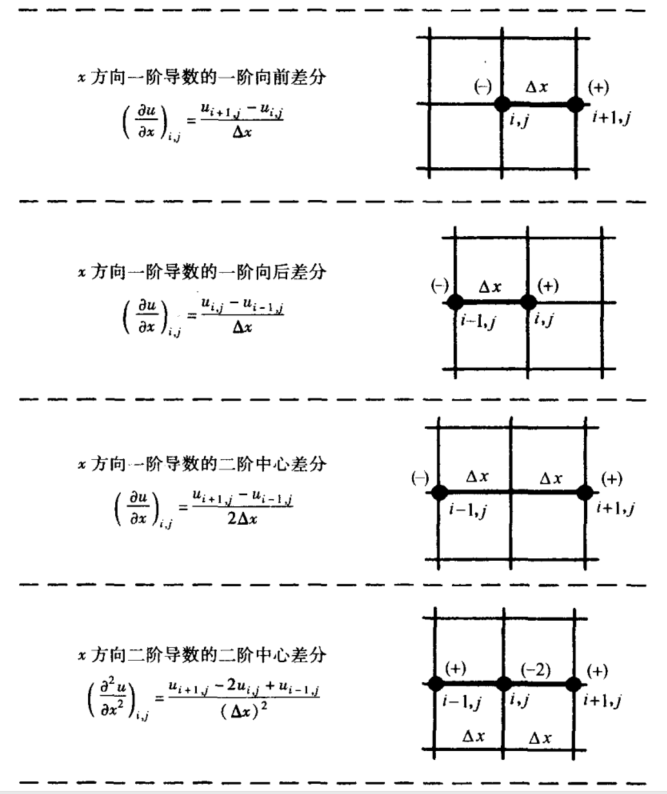
\includegraphics[width=0.7\linewidth]{figures/youxianchafentujie.png}
	\caption{youxianchafentujie}
	\label{fig:youxianchafentujie}
\end{figure}

\begin{figure}
	\centering
	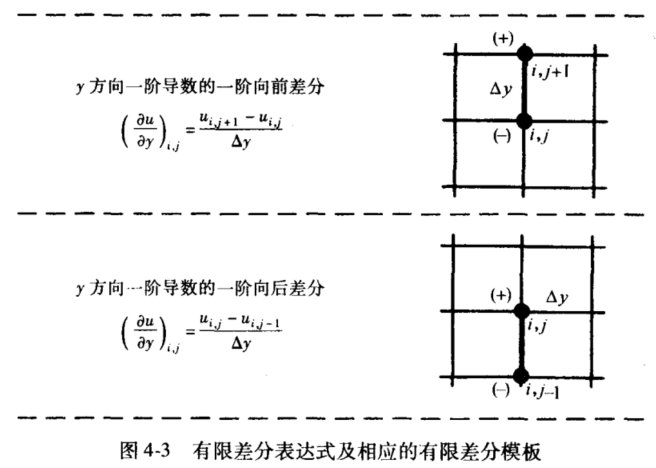
\includegraphics[width=0.7\linewidth]{figures/youxianchafentujie2.png}
	\caption{youxianchafentujie2}
	\label{fig:youxianchafentujie2}
\end{figure}

\begin{figure}
	\centering
	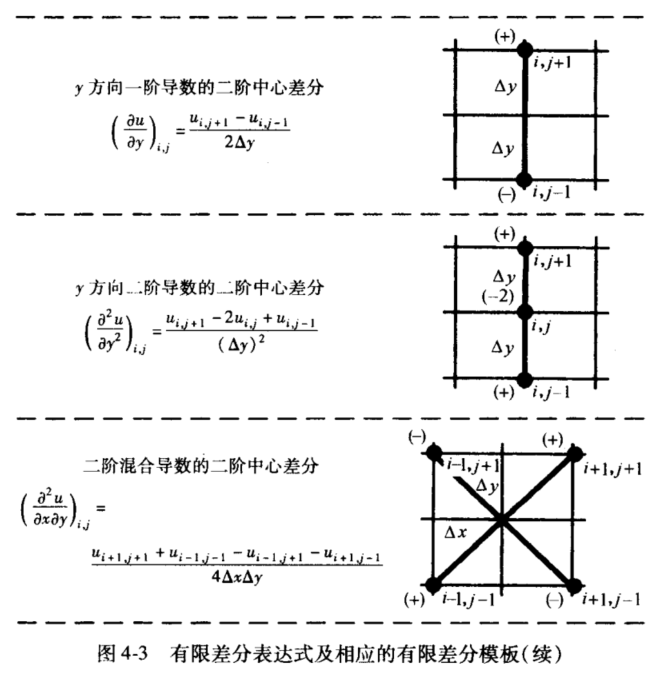
\includegraphics[width=0.7\linewidth]{figures/youxianchafentujie3.png}
	\caption{youxianchafentujie3}
	\label{fig:youxianchafentujie3}
\end{figure}


\subsection{边界处理}
1. 使用 假设边界的下面的值就等于边界的值来回避这个问题

2. 使用多项式近似的方法来对边界值进行求解

\subsection{显式方法}
显式方法中每一个差分方程只包含一个未知数, 从而这个未知数可以用直接计算的方式显式地求解.

优点: 方法的建立及编程相对简单

缺点: 更具上面的例子, 对确定的$\Delta  x$,  $\Delta t$ 要尽量小, 否则容易出现不稳定状态, 导致了计算时间耗时较长.
\subsection{隐式方法}
对于排列在同一时间层所有网格点上的未知量, 必须将它们联立起来同时求解, 才能求出这些未知量. -- 采用追赶法, 托马斯算法.

优点: 耗时更小, $\Delta t$ 显示的更加稳定

缺点: 方法的建立和编程更复杂.

\subsection{波数}
下标m的含义, 它就等于给定区间包含的波形的个数.


\subsection{稳定解判定}
$$
	\left|\frac{\varepsilon_{i}^{n+1}}{\varepsilon_{i}^{n}}\right|=\left|\mathrm{e}^{\alpha \Delta t}\right|=\left|1-\frac{4 \alpha \Delta t}{(\Delta x)^{2}} \sin ^{2} \frac{k_{m} \Delta x}{2}\right| \leqslant 1
$$

分析方法, 冯诺伊曼稳定性方法.

柯朗-弗里德里奇-列为条件, 这个天剑对于双曲型方程来说是一个重要的稳定性准则. 要保证稳定性, 数值解的依赖区域必须全部包含解析解的依赖区域.

\subsection{网格变换}
简单的来说就是建立一个联系, 将物理坐标和计算坐标建立联系

$$
	\frac{\partial}{\partial x}=\left(\frac{\partial}{\partial \xi}\right)\left(\frac{\partial \xi}{\partial x}\right)+\left(\frac{\partial}{\partial \eta}\right)\left(\frac{\partial \eta}{\partial x}\right)
$$

$$
	\frac{\partial}{\partial y}=\left(\frac{\partial}{\partial \xi}\right)\left(\frac{\partial \xi}{\partial y}\right)+\left(\frac{\partial}{\partial \eta}\right)\left(\frac{\partial \eta}{\partial y}\right)
$$

$$
	\frac{\partial}{\partial t}=\left(\frac{\partial}{\partial \xi}\right)\left(\frac{\partial \xi}{\partial t}\right)+\left(\frac{\partial}{\partial \eta}\right)\left(\frac{\partial \eta}{\partial t}\right)+\left(\frac{\partial}{\partial \tau}\right)\left(\frac{\mathrm{d} \tau}{\mathrm{d} t}\right)
$$

$$
	\begin{aligned}
		\frac{\partial^{2}}{\partial x^{2}}= & \left(\frac{\partial}{\partial \xi}\right)\left(\frac{\partial^{2} \xi}{\partial x^{2}}\right)+\left(\frac{\partial}{\partial \eta}\right)\left(\frac{\partial^{2} \eta}{\partial x^{2}}\right)+\left(\frac{\partial^{2}}{\partial \xi^{2}}\right)\left(\frac{\partial \xi}{\partial x}\right)^{2}+\left(\frac{\partial^{2}}{\partial \eta^{2}}\right)\left(\frac{\partial \eta}{\partial x}\right)^{2}+ \\
		                                     & 2\left(\frac{\partial^{2}}{\partial \eta \partial \xi}\right)\left(\frac{\partial \eta}{\partial x}\right)\left(\frac{\partial \xi}{\partial x}\right)
	\end{aligned}
$$

$$
	\begin{aligned}
		\frac{\partial^{2}}{\partial y^{2}}= & \left(\frac{\partial}{\partial \xi}\right)\left(\frac{\partial^{2} \xi}{\partial y^{2}}\right)+\left(\frac{\partial}{\partial \eta}\right)\left(\frac{\partial^{2} \eta}{\partial y^{2}}\right)+\left(\frac{\partial^{2}}{\partial \xi^{2}}\right)\left(\frac{\partial \xi}{\partial y}\right)^{2}+ \\
		                                     & \left(\frac{\partial^{2}}{\partial \eta^{2}}\right)\left(\frac{\partial \eta}{\partial y}\right)^{2}+2\left(\frac{\partial^{2}}{\partial \eta \partial \xi}\right)\left(\frac{\partial \eta}{\partial y}\right)\left(\frac{\partial \xi}{\partial y}\right)
	\end{aligned}
$$

$$
	\begin{aligned}
		\frac{\partial^{2}}{\partial x \partial y}=\left(\frac{\partial}{\partial \xi}\right)\left(\frac{\partial^{2} \xi}{\partial x \partial y}\right)+\left(\frac{\partial}{\partial \eta}\right)\left(\frac{\partial^{2} \eta}{\partial x \partial y}\right)+\left(\frac{\partial^{2}}{\partial \xi^{2}}\right)\left(\frac{\partial \xi}{\partial x}\right)\left(\frac{\partial \xi}{\partial y}\right)+ \\
		\left(\frac{\partial^{2}}{\partial \eta^{2}}\right)\left(\frac{\partial \eta}{\partial x}\right)\left(\frac{\partial \eta}{\partial y}\right)+\left(\frac{\partial^{2}}{\partial \xi \partial \eta}\right)\left[\left(\frac{\partial \eta}{\partial x}\right)\left(\frac{\partial \xi}{\partial y}\right)+\left(\frac{\partial \xi}{\partial x}\right)\left(\frac{\partial \eta}{\partial y}\right)\right]
	\end{aligned}
$$

因为比较复杂, 使用逆度量来减少复杂度

$$
	\frac{\partial}{\partial x}=\frac{1}{J}\left[\left(\frac{\partial}{\partial \xi}\right)\left(\frac{\partial y}{\partial \eta}\right)-\left(\frac{\partial}{\partial \eta}\right)\left(\frac{\partial y}{\partial \xi}\right)\right]
$$

$$
	\frac{\partial}{\partial y}=\frac{1}{J}\left[\left(\frac{\partial}{\partial \eta}\right)\left(\frac{\partial x}{\partial \xi}\right)-\left(\frac{\partial}{\partial \xi}\right)\left(\frac{\partial x}{\partial \eta}\right)\right]
$$

$$
	\begin{aligned}
		 & \frac{\partial \xi}{\partial x}=\frac{1}{J} \frac{\partial y}{\partial \eta}  \\
		 & \frac{\partial \eta}{\partial x}=-\frac{1}{J} \frac{\partial y}{\partial \xi} \\
		 & \frac{\partial \xi}{\partial y}=-\frac{1}{J} \frac{\partial x}{\partial \eta} \\
		 & \frac{\partial \eta}{\partial y}=\frac{1}{J} \frac{\partial x}{\partial \xi}
	\end{aligned}
$$

\subsection{自适应网格}
1. 当网格数量固定时, 可以提高计算精度

2. 给定精度时, 可以用较少的网格点来达到这一精度.

笛卡尔积网格, 网格靠近物体的边界直接向物体拟合.


\subsection{显示有限差分方法}
1. 拉克斯-温德罗夫Lax-Wendroff方法

2. 麦考马克(MacCormack)方法

最容易理解和编程的方法之一.

应用于非定常纳维-斯托克斯方程的求解.

3. 松弛法

如果截断误差的主项是偶数阶导数, 数值解将主要表现出耗散行为; 如果主项是奇数阶导数, 数值解将主要表现出色散行为.

人工粘性加入可以得到一个稳定的解.



$$
	\begin{aligned}
		 & \overline{S_{i, j}^{t+\Delta t}}=C_{x} \frac{\left|\overline{p_{i+1, j}^{t+\Delta t}}-2 \overline{p_{i, j}^{t+\Delta t}}+\overline{p_{i-1, j}^{t+\Delta t}}\right|}{\overline{p_{i+1, j}^{t+\Delta t}}+2 \overline{p_{i, j}^{t+\Delta t}}+\overline{p_{i-1, j}^{t+\Delta t}}}\left(\overline{U_{i+1, j}^{t+\Delta t}}-2 \overline{U_{i, j}^{t+\Delta}}+\overline{U_{i-1, j}^{t+\Delta t}}\right)+ \\
		 & C_{y} \frac{\left|\bar{p}_{i, j+1}^{t+\Delta t}-2 \bar{p}_{i, j}^{t+\Delta t}+\overline{p_{i, j-1}^{t+\Delta t}}\right|}{p_{i, j+1}^{t+\Delta t}+2 \overline{p_{i, j}^{t+\Delta x}}+\overline{p_{i, j-1}^{t+\Delta t}}}\left(\overline{U_{i, j+1}^{t+\Delta t}}-2 \overline{U_{i, j}^{t+\Delta t}}+\overline{U_{i, j-1}^{t+\Delta t}}\right)
	\end{aligned}
$$
\subsection{交替方向隐式(ADI)方法}


简单的说, 将不能使用, 托马斯方法的矩阵变成可以使用托马斯方法??

\subsection{压力修正法}
不可压纳维-斯托克斯方程

$$
	\begin{array}{|lc|}
		\hline \text { 连续性方程 } & \nabla \cdot V=0                                                                                  \\
		x \text { 方向动量方程 }    & \rho \frac{\mathrm{D} u}{\mathrm{D} t}=-\frac{\partial p}{\partial x}+\mu \nabla^{2} u+\rho f_{x} \\
		y \text { 方向动量方程 }    & \rho \frac{\mathrm{D} v}{\mathrm{D} t}=-\frac{\partial p}{\partial y}+\mu \nabla^{2} v+\rho f_{y} \\
		z \text { 方向动量方程 }    & \rho \frac{\mathrm{D} w}{\mathrm{D} t}=-\frac{\partial p}{\partial z}+\mu \nabla^{2} w+\rho f_{z}
	\end{array}
$$

迎风差分. 简答说就是在不同位置就算u, 在不同位置计算v.

\subsection{数值方法: SIMPLE算法}
Semi-implicit method for pressure-linked equations(压力耦合方程的半隐式算法)


\subsection{马赫数}
马赫数(Ma)

这是流体力学中表征流体可压缩程度的一个重要的无量纲参数,记为Ma,定义为流场中某点的速度v 同该点的当地声速c 之比,它是以奥地利科学家E.马赫的姓氏命名的。

$$
	Ma = \frac{v}{c}
$$

由定义可知,马赫数是表示声速倍数的数,一马赫即一倍音速:马赫数小于1者为亚音速,近乎等于1为跨声速,大于1为超声速。

\section{计算流体力学视频}
\url{https://www.bilibili.com/video/BV1vE411W7kV?from=search&seid=17354358762961406319&spm_id_from=333.337.0.0}